\normalfont\normalsize
\chapter{Implementation}

This chapter presents some aspects of the implementation worth mentioning. Some parts of the tasks running on the wireless sensors,
how the algorithm for the scheduler is implemented.

\section{Tasks}

This section presents some archetypes of Contiki tasks, most of the tasks needed for a WSN application as described in this
study can be implemented from this basis. We include parts of the metatask, one of the tasks that monitor the node and 
a framework for a sensing task.

\subsection{Metatask}

The meta-task is the process on each sensor node responsible for task management. It is implemented as a server, any incoming connection
is treated as a sequence of commands to start/stop or modify the tasks. Nodes begin with a list of implemented tasks predefined (in
agreement with their capabilities). The meta-task is automatically started on each reset and maintains a list of the other tasks and their
status.
\begin{figure}[ht]
 \begin{center}
  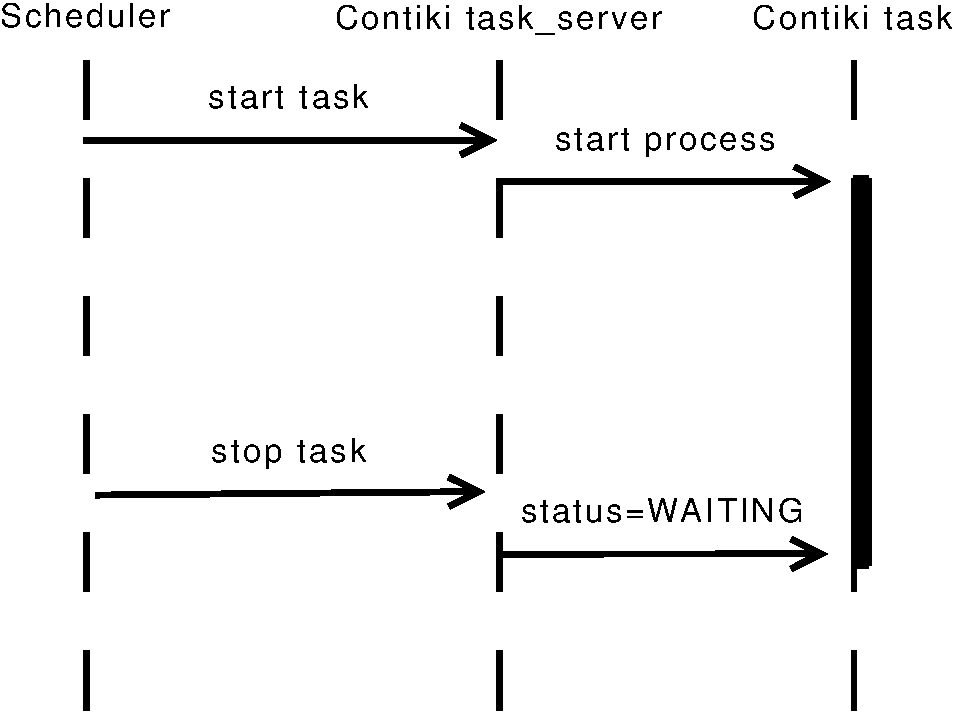
\includegraphics[scale=0.5]{implementation/start_task.pdf}
 \end{center}
 \caption{\small \itshape{The exchange of messages while starting/stopping tasks}}
\end{figure}

\begin{figure}[ht]
 \begin{center}
  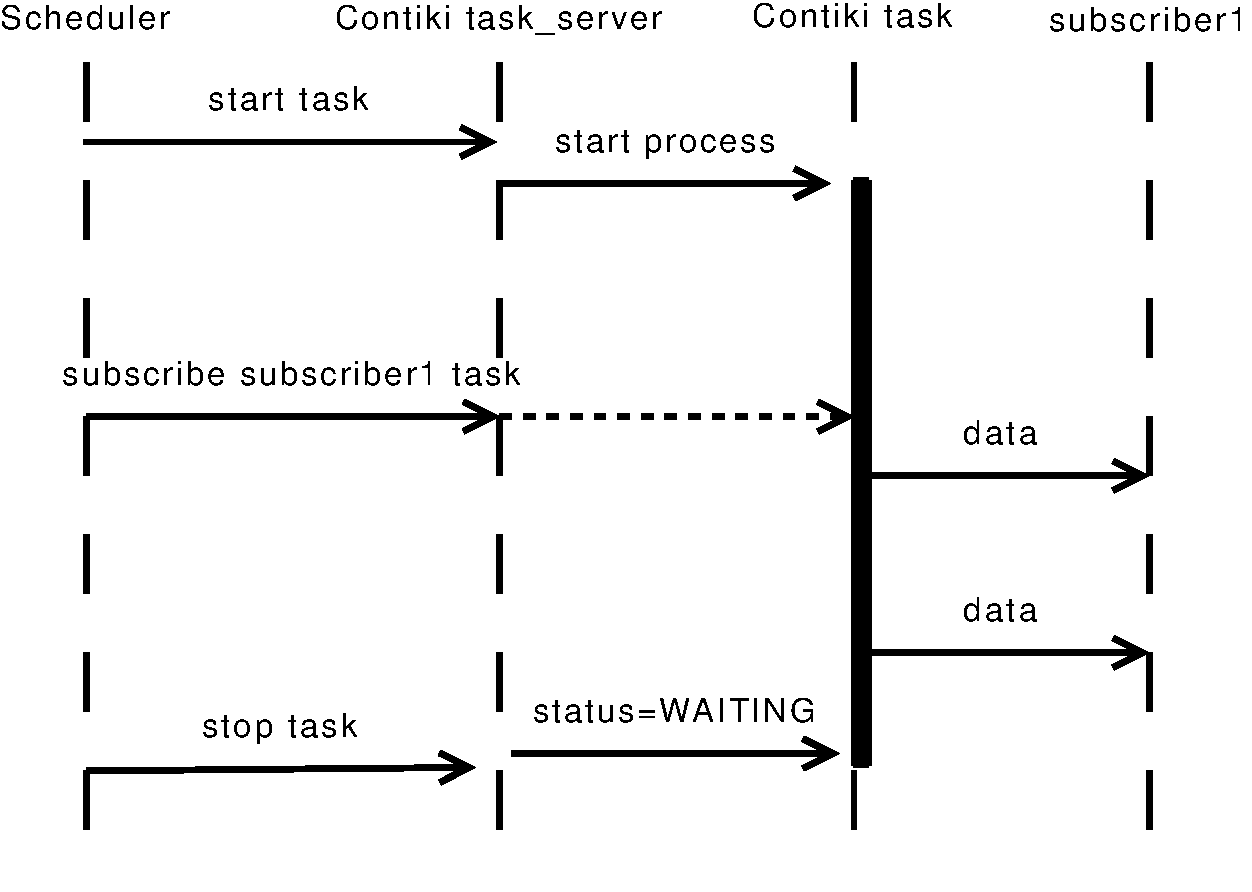
\includegraphics[scale=0.5]{implementation/subscribe.pdf}
 \end{center}
 \caption{\small \itshape{The exchange of message during subscription of a task on another node to the output of a task on the current node}}
\end{figure}

\lstset{numbers=left, mathescape=true, nolol=false,caption=Task server snippet,label=lst:taskserver}
\begin{lstlisting}
PROCESS_THREAD(task_server_process, ev, data)
{
	PROCESS_BEGIN();

	list_init(task_list);

	list_add(task_list,&el_monitor_process);
	list_add(task_list,&el_delay_process);
	list_add(task_list,&el_temperature_sensing);

	tcp_listen(HTONS(1010));

	while(1) 
	{
		PROCESS_WAIT_EVENT_UNTIL(ev == tcpip_event);

		if(uip_connected()) 
		{
			PSOCK_INIT(&ps, buffer, sizeof(buffer));

			while(!(uip_aborted() || uip_closed() 
			    || uip_timedout())) 
			{
				PROCESS_WAIT_EVENT_UNTIL
				      (ev == tcpip_event);
				handle_connection(&ps);
			}
		}
	}
	PROCESS_END();
}
\end{lstlisting}
\subsection{Load monitor process}

The load monitor is the tool discussed in \ref{sec:nodeload}, which helps determine whether a node can take extra processes or not.
Generally we believe that a collaborative system will have a maximum number of tasks, highly dependendant on the programming
of each one, of their frequencies of communication, activity and so on. This metric might also be called a responsiveness metric,
the value is the time between schedules.

\lstset{numbers=left, mathescape=true, nolol=false,caption=Load monitor process,label=lst:loadmonitor}
\begin{lstlisting}
PROCESS_THREAD(monitor_process, ev, data)
{
	PROCESS_BEGIN();
	while(1)
	{
		t1 = clock_time();
		PROCESS_PAUSE();
		dif = clock_time() - t1;
	}
	
	PROCESS_END();
}
\end{lstlisting}
\subsection{Sensing Task}
\lstset{numbers=left, mathescape=true, nolol=false,caption=Sensing taks (generic) snippet,label=lst:sensingtask}
\begin{lstlisting}
\small
PROCESS_THREAD(sensing_process, ev, data)
{
	PROCESS_BEGIN();

	while(1) 
	{
		tatic struct etimer et;
  
  
		etimer_set(&et, CLOCK_SECOND * 10);
		PROCESS_WAIT_EVENT();

		if(etimer_expired(&et)) 
		{
			while(tc.forwarding) 
			{
				PROCESS_PAUSE();
 			}

			for(i = 0; i < el_sensing_process.nrsub; i++)
			{
				/* form the IPv6 address */
				uip_ip6addr(paddr,
					el_sensing_process.sub[i][0],
					el_sensing_process.sub[i][1],
					el_sensing_process.sub[i][2],
					el_sensing_process.sub[i][3],
					el_sensing_process.sub[i][4],
					el_sensing_process.sub[i][5],
					el_sensing_process.sub[i][6],
					el_sensing_process.sub[i][7]);
				tcp_connect(paddr,HTONS(4242),NULL);

				PROCESS_WAIT_EVENT_UNTIL
				    (ev ==tcpip.event);

				if (uip_connected())
				{
					PSOCK_INIT(
					  &el_sensing_process.protosock,
					  buffer,sizeof(buffer));

					do
					{
						handle_send(&ps2);
					}while (!(uip_close() || 
						uip_aborted() ||
						uip_timedout()));
				}
			}
		}
	}
	PROCESS_END();
}
\end{lstlisting}
\section{Scheduler}

The scheduler itself is currently written in Python. Python was chosen for its ease of development and higher-level primitive 
data types that are well suited for more complex algorithms such as this one.

The scheduler uses pygraph as a framework for basic graph operations (adding edges, removing nodes, etc.), and graphviz for 
visualising data. 

\lstset{numbers=left, mathescape=true, nolol=false,caption=Main K-Cut algorithm,label=lst:kcutimpl}
\begin{lstlisting}
def kcut(graph,k):
	kp= k - 2 + (k % 2)
	if kp < 1:
		kp = 1
	if k == 1:
		return [graph.nodes()]

	#tasks that have multiplicity
	mt = [e for e in graph.nodes() 
		if tasks[e]['multiplicity']>1]

	st = affine_possibilities(
	    list(set(graph.nodes()).difference(set(mt))),
	    kp,
	    len(battery)-k)
	tt = possibilities(graph.nodes(),k-1)

	mincut = []
	for s in st:
		for t in tt:
			if len(set(s).intersection(set(t))) == 0:
				res = stcut(graph,s,t)
				if len(mincut)==0:
					mincut = res
				else:
					if res[2] < mincut[2]:
						mincut = res
	for old in mincut[0]:
		graph.del_node(old)
	return [mincut[0]+mt] + kcut(graph,k-1)

\end{lstlisting}

